\documentclass[18pt]{beamer}
\usepackage{templates/beamerthemekit}
\usepackage[export]{adjustbox}
\usepackage{tikz}
% \usepackage{templates/beamerthemekitwide}

%\titlelogo{mylogo}
% \usepackage{templates/tikzkit}
% \usepackage{templates/tikzuml}
%\titleimage{myimage}
\titlelogo{myimage}


\title[Short title]{Erstellung und Evaluierung stochastischer Regressionsmodelle auf Basis heterogener Messnetzwerke.}
\subtitle{Bachelor Arbeit, Betreuer - Dr. Johannes Riesterer, Dr. Sebastian Lerch}
\author{Stanislav Arnaudov}

\institute{TECO - Das Telecooperation Office}
\usepackage[citestyle=authoryear,bibstyle=numeric,hyperref,backend=biber]{biblatex}
\addbibresource{templates/example.bib}
\bibhang1em
 
\begin{document} 

% \selectlanguage{english}
\selectlanguage{ngerman}


\begin{frame}
 \titlepage
\end{frame}

\begin{frame}
  \frametitle{Motivation}
  
  \begin{columns}
    \begin{column}{0.4\textwidth}
      Probleme:
      \begin{itemize}
      \item Verbesserung von Regressionsmodellen für Sensornetze  durch Hinzunahme unsicherer Sensoren.
      \item Automatische Qualitätsbestimmung der Sensoren eines Sensornetzes.
      \item Die Genauigkeit bei Messen durch Berücksichtigung der Unsicherheit erhöhen.
      \end{itemize}
    \end{column}
    \begin{column}{0.6\textwidth}
      \begin{center}
        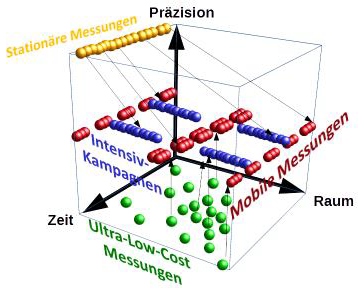
\includegraphics[scale=0.5]{images/motivation}
      \end{center}
    \end{column}
  \end{columns}
  
\end{frame}

\begin{frame}
  \frametitle{Daten}
  \begin{itemize}
  \item Heterogenes Netzwerk von Feinstaubsensoren in Stuttgart.\\
  \item Daten aus:
    \begin{itemize}
    \item LU-BW (\textit{Landesanstalt für Umwelt, Messungen und Naturschutz Baden-Württemberg}) - \textbf{3 Sensoren} hocher Qualität.
    \item \textit{luftdaten.info} -- Daten aus einer großen Menge unsicherer Sensoren.
    \end{itemize}
  \item Zeitraum: von 2017 bis jetzt.
  \end{itemize}

  \begin{columns}
    \begin{column}{0.5\textwidth}
      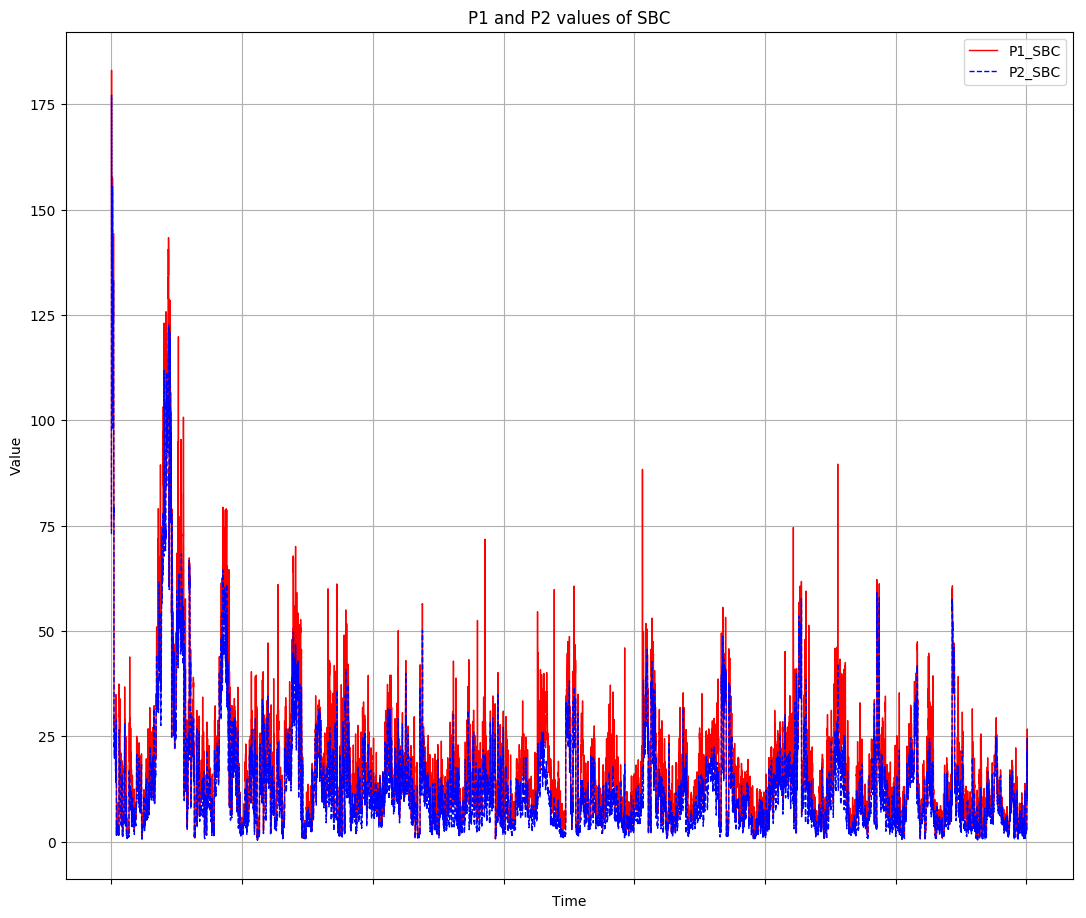
\includegraphics[scale=0.2]{images/SBC_1}
    \end{column}
    \begin{column}{0.5\textwidth}
      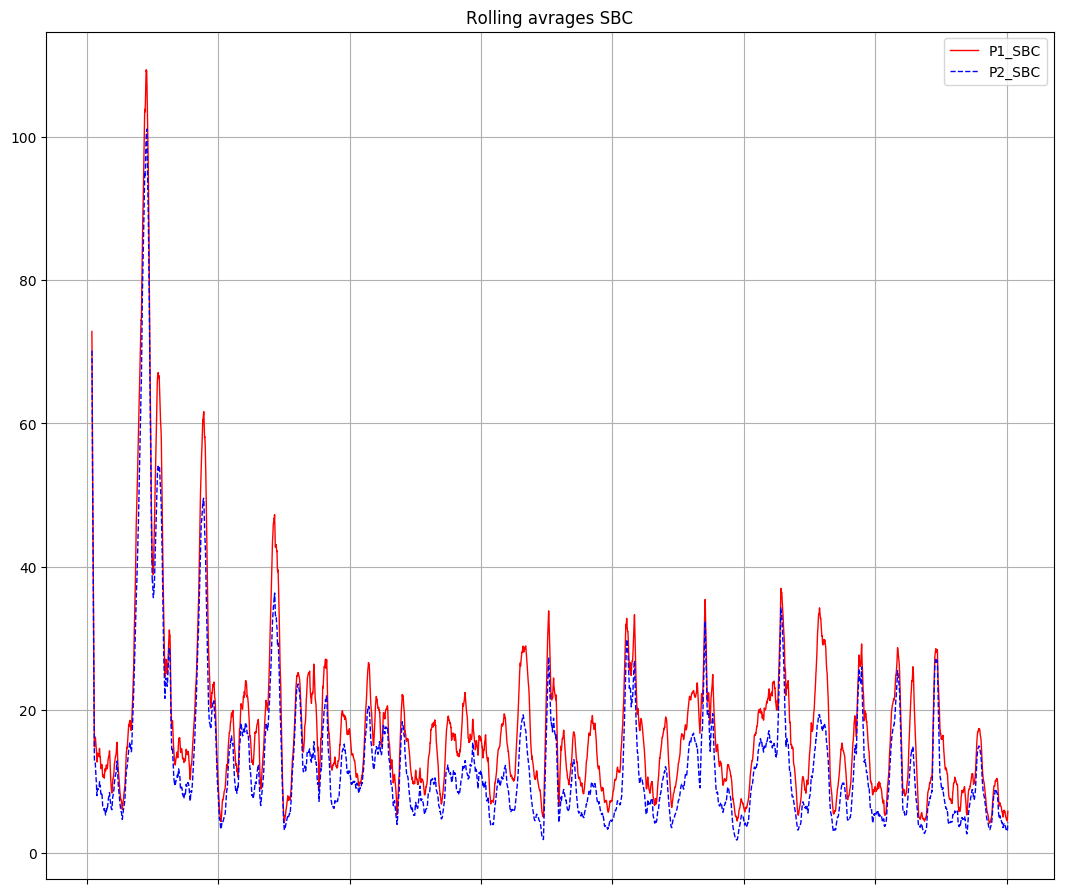
\includegraphics[scale=0.2]{images/SBC_2}
    \end{column}
  \end{columns}

\end{frame}

\begin{frame}
  \frametitle{Stochastische Regressionsmodelle}
    \begin{columns}
      \begin{column}{0.35\textwidth}
        \begin{itemize}
        \item Bayesian Neural Networks
          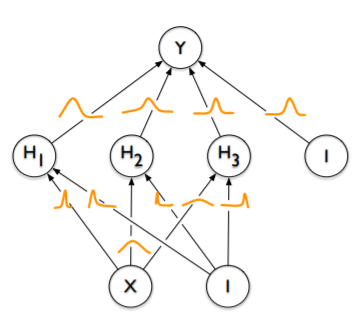
\includegraphics[scale=0.35]{images/bnn}
        \end{itemize}
    \end{column}
    \begin{column}{0.65\textwidth}
      \begin{itemize}
      \item Mixtures of Gaussian Process Experts
          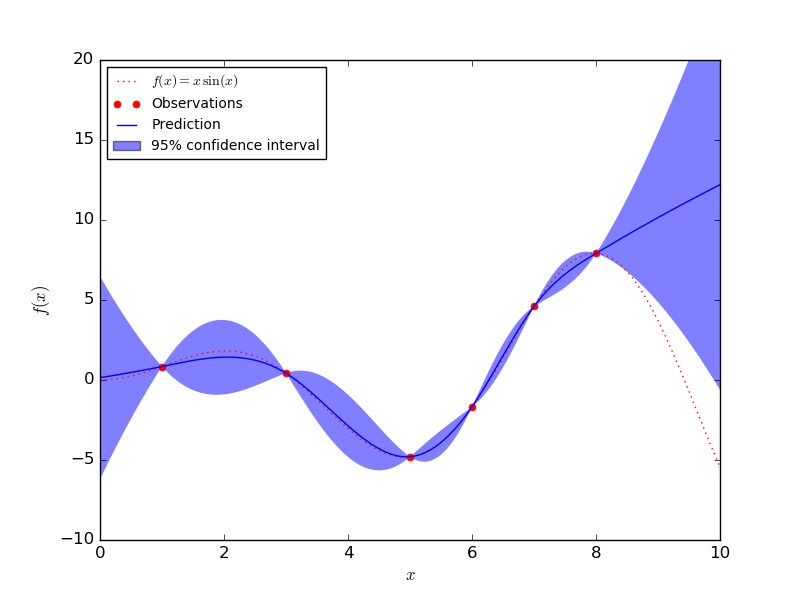
\includegraphics[scale=0.3]{images/graph_1}
      \end{itemize}
    \end{column}
  \end{columns}
\end{frame}

\begin{frame}
  \frametitle{Trainieren}
  
    \begin{itemize}
    \item Trainieren mit Zeitreihen von allen Sensoren.

      \begin{tikzpicture}[yscale=-1] 
        \draw (0, 0) grid (5, 5);
        \draw [color=black, fill=black] (0, 0) circle (0.1);

        \draw [color=blue, fill=blue] (1, 1) circle (0.1);
        \draw [color=blue, fill=blue] (2, 4) circle (0.1);
        \draw [color=blue, fill=blue] (4, 2) circle (0.1);
        
        \draw [color=red, fill=red] (1.5, 1.5) circle (0.05);
        \draw [color=red, fill=red] (1.5, 3.5) circle (0.05);
        \draw [color=red, fill=red] (3.5, 1.5) circle (0.05);
        \draw [color=red, fill=red] (3, 1) circle (0.05);
        \draw [color=red, fill=red] (2, 2) circle (0.05);
        \draw [color=red, fill=red] (4, 4) circle (0.05);
        \draw [color=red, fill=red] (3, 3) circle (0.05);
        \draw [color=red, fill=red] (3.5, 3.5) circle (0.05);
        \draw [color=red, fill=red] (2.5, 3.5) circle (0.05);
        \draw [color=red, fill=red] (0.5, 0.5) circle (0.05);
        \draw [color=red, fill=red] (3, 2) circle (0.05);
        \draw [color=red, fill=red] (1, 2) circle (0.05);
        \draw [color=red, fill=red] (1, 2.5) circle (0.05);
        \draw [color=red, fill=red] (4, 2.5) circle (0.05);
        \draw [color=red, fill=red] (2.5, 0.5) circle (0.05);
        \draw [color=red, fill=red] (2, 4.5) circle (0.05);

        \node[inner sep=0pt]  at (2.75,4.75)
        {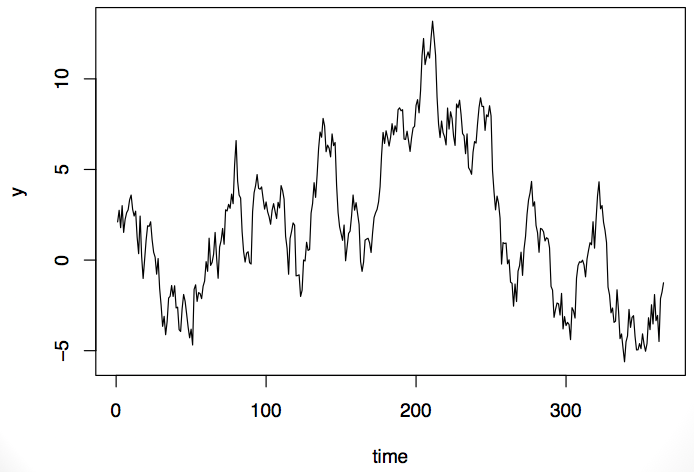
\includegraphics[width=.1\textwidth]{images/ts}};
        \node[inner sep=0pt]  at (0.75,4.00)
        {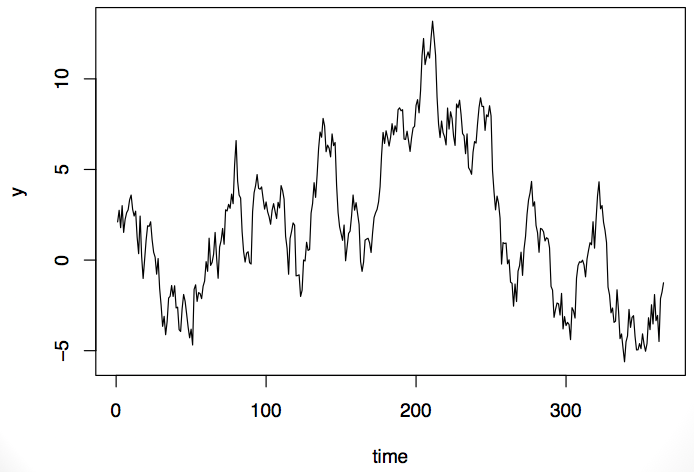
\includegraphics[width=.1\textwidth]{images/ts}};
        \node[inner sep=0pt]  at (4.5,4.5)
        {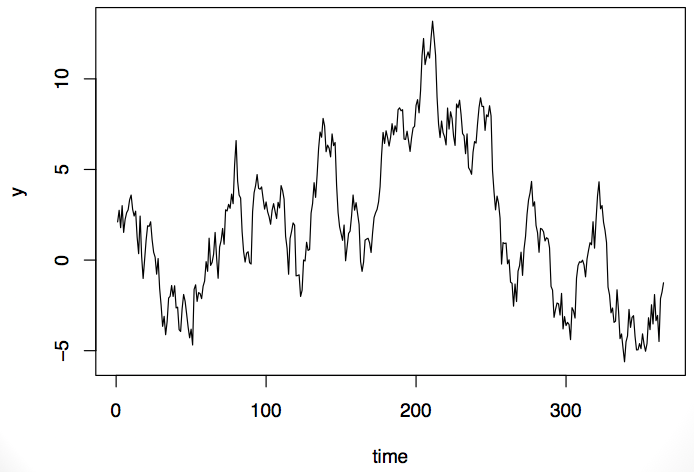
\includegraphics[width=.1\textwidth]{images/ts}};
        \node[inner sep=0pt]  at (4.5,3)
        {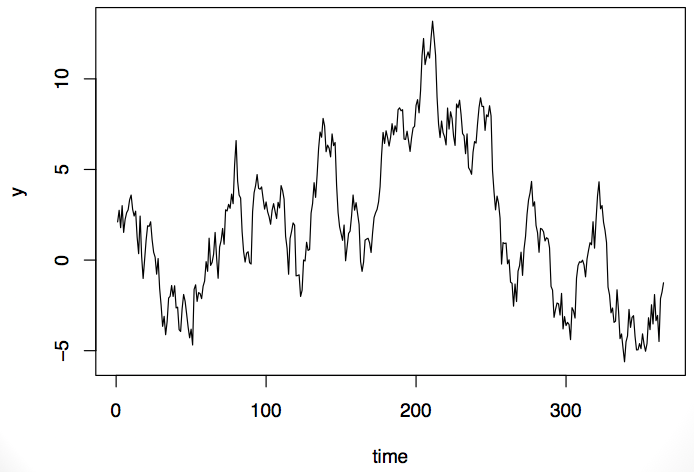
\includegraphics[width=.1\textwidth]{images/ts}};
        \node[inner sep=0pt]  at (3.8,1)
        {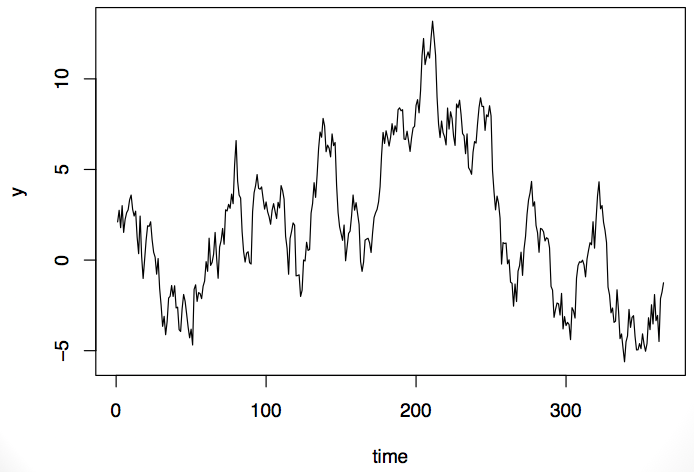
\includegraphics[width=.1\textwidth]{images/ts}};
        
        \draw[ thick, ->] (1.5,1.5) parabola (1,1);
        \draw[ thick, ->] (1.5,3.5) parabola (1,1);
        \draw[ thick, ->] (4,4) parabola (1,1);
        \draw[ thick, ->] (3,2) parabola (1,1);
        \draw[ thick, ->] (4,2.5) parabola (1,1);
        \draw[ thick, ->] (3.5,1.5) parabola (1,1);
        \draw[ thick, ->] (4, 2) parabola (1,1);
        \draw[ thick, ->] (2, 4) parabola (1,1);
        
        \draw[ thick, ->] (1,1) .. controls (3,0) and (5,0) .. (7,1);

        \node[] at (6.8,1.25) {Wahrscheinlichkeitsverteilung};
        \node[inner sep=0pt]  at (6.8,2.25)
        {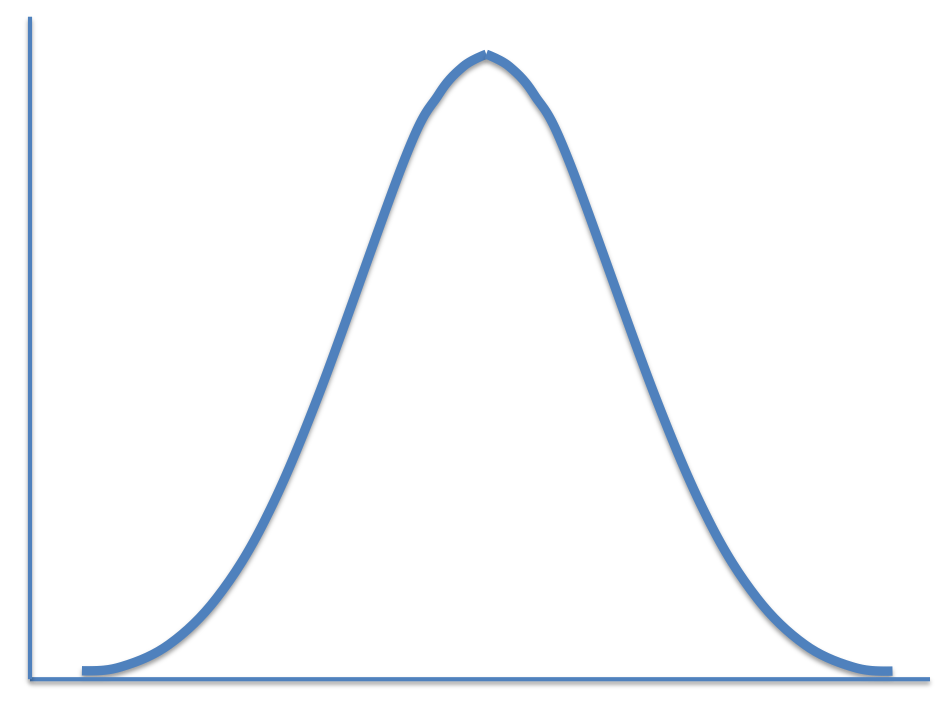
\includegraphics[width=.2\textwidth]{images/pdf}};
        
        \draw [thick,->] (0, 0) -- (5, 0);
        \draw [thick,->] (0, 0) -- (0, 5);
        \node at (-0.1, -0.5) {(0, 0)};
        \node at (4.5, -0.5) {lat.};
        \node at (-0.5, 5) {lon.};
        
        \node[] at (-1,0) {LU-BW};
        \draw [color=blue, fill=blue] (-1.75 , 0) circle (0.1);
        \node[] at (-1,1) {luftdaten.info};
        \draw [color=red, fill=red] (-2.2 , 1) circle (0.1);
        
      \end{tikzpicture}
      
    \item  Loss Functions -- Wahrscheinlichkeitsverteilungen.
    \end{itemize}
  
\end{frame}

\begin{frame}
  \frametitle{BNN mit Edward und Tesorflow}
  \begin{columns}
    \begin{column}{0.4\textwidth}
      \begin{itemize}
      \item Daten - Kosinus mit Rauschen
      \item Zweidimensionaler Eingaberaum: $z = cos(x_1 + x_2) + \epsilon, \newline \epsilon\sim N(0, 0.5)$
      \item Eindimensionale Repräsentation 
        \begin{itemize}
        \item Auswerten vom Modell über die Eingabedaten
        \item X-Achse - Index vom entsprechenden Datenpunkt
        \end{itemize} 
      \end{itemize}
    \end{column}
    \begin{column}{0.6\textwidth}
      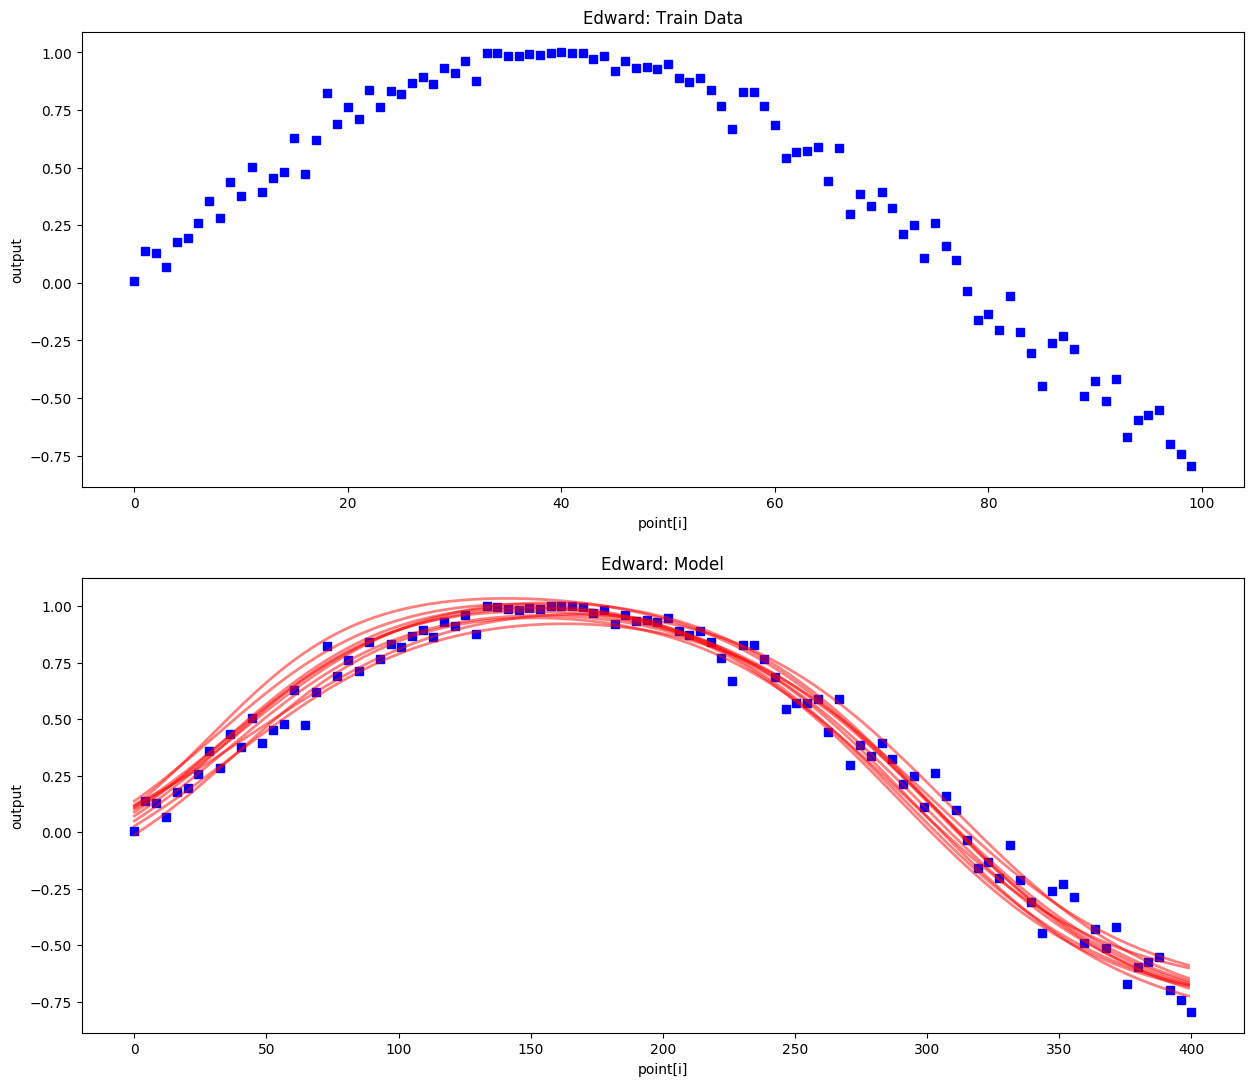
\includegraphics[scale=0.2]{images/edward_example_bnn}
    \end{column}
  \end{columns}
  
\end{frame}

\begin{frame}
  \frametitle{Evaluierung von Modellen}
  \begin{columns}
    \begin{column}{0.5\textwidth}
      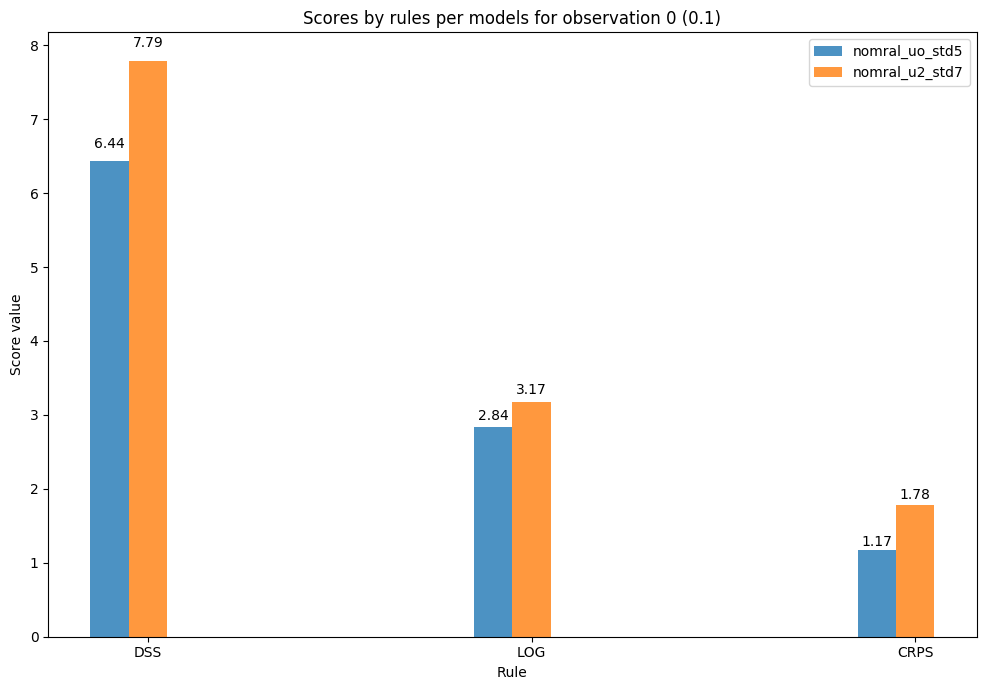
\includegraphics[scale=0.2]{images/cross_model_scoring_0}
      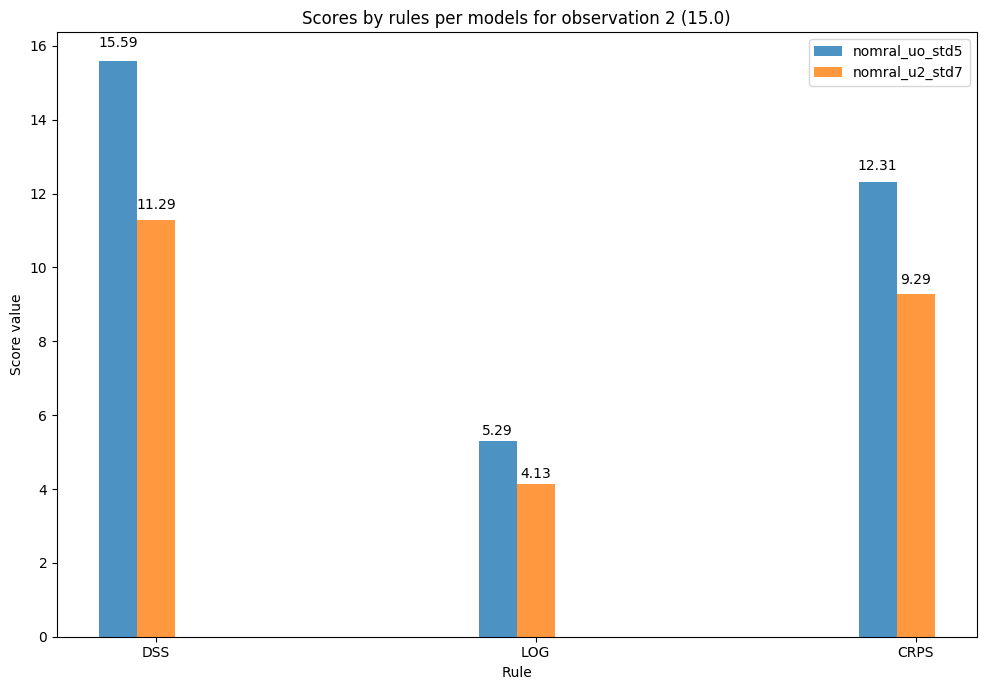
\includegraphics[scale=0.2]{images/cross_model_scoring_2}
    \end{column}
    \begin{column}{0.5\textwidth}
      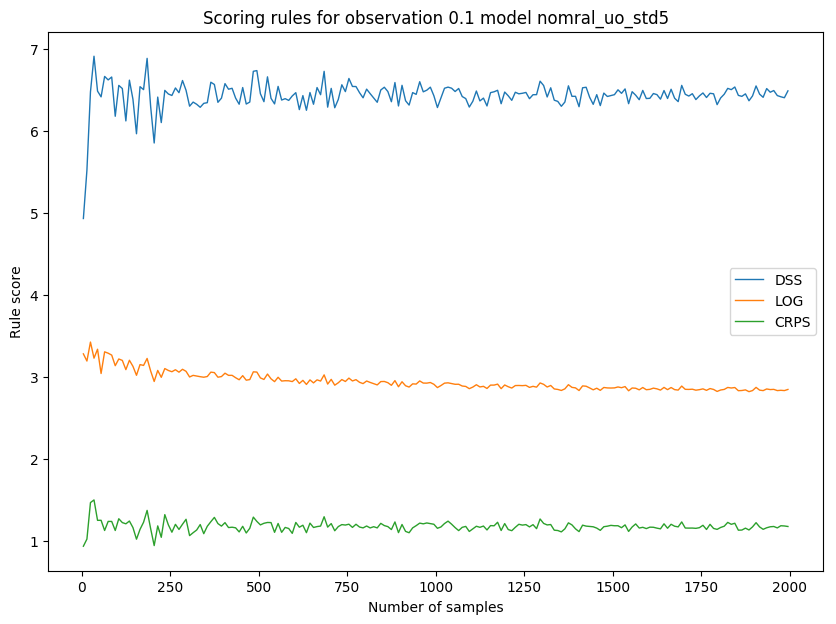
\includegraphics[scale=0.23]{images/scroring_nomral_uo_std5_0}
      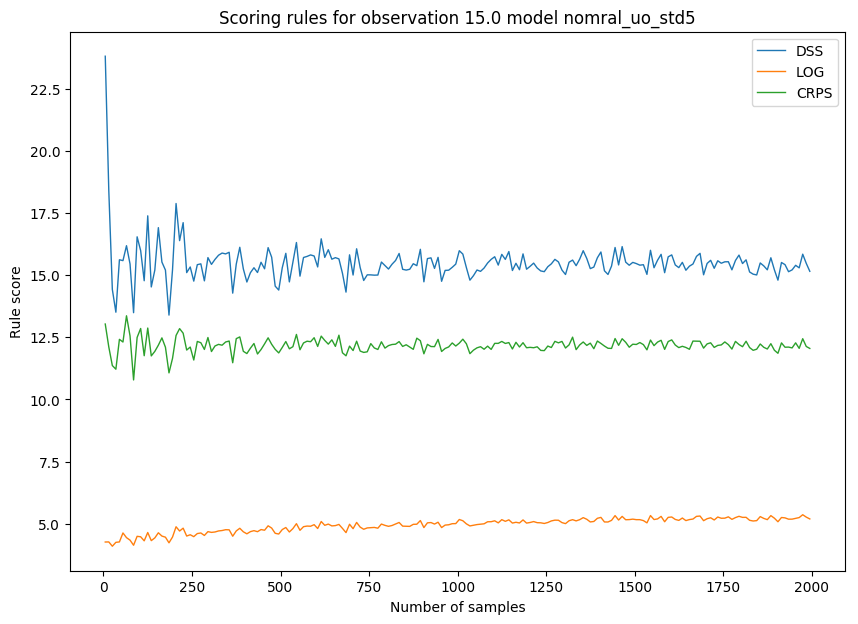
\includegraphics[scale=0.23]{images/scroring_nomral_uo_std5_2}
    \end{column}
  \end{columns}
\end{frame}


\end{document}

%%% Local Variables:
%%% mode: latex
%%% TeX-master: t
%%% End:
